%allgemeine Formatangaben
\documentclass[
 a4paper, 										% Papierformat
 12pt,												% Schriftgröße
 ngerman, 										% für Umlaute, Silbentrennung etc.
 %titlepage,										% es wird eine Titelseite verwendet
 oneside, 										% einseitiges Dokument
 captions=nooneline,					% einzeilige Gleitobjekttitel ohne Sonderbehandlung wie mehrzeilige Gleitobjekttitel behandeln
 numbers=noenddot,						% Überschriften-??Nummerierung ohne Punkt am Ende
 parskip=half,									% zwischen Absätzen wird eine halbe Zeile eingefügt
 ]{scrartcl}

% Anpassung an Landessprache
\usepackage[ngerman]{babel}	

\usepackage[T1]{fontenc}	
\usepackage[utf8]{inputenc}	
\usepackage{textcomp} 																% Euro-Zeichen und andere
\usepackage[babel,german=quotes]{csquotes}						% Anführungszeichen
\RequirePackage[ngerman=ngerman-x-latest]{hyphsubst} 	% erweiterte Silbentrennung

% Befehle aus AMSTeX für mathematische Symbole z.B. \boldsymbol \mathbb
\usepackage{amsmath,amsfonts}

% Zeilenabstände und Seitenränder 
\usepackage{setspace}
\usepackage{geometry}

% Einbinden von JPG-Grafiken
\usepackage{graphicx}

% zum Umfließen von Bildern
% Verwendung unter http://de.wikibooks.org/wiki/LaTeX-Kompendium:_Baukastensystem#textumflossene_Bilder
\usepackage{floatflt}

% Verwendung von vordefinierten Farbnamen zur Colorierung
% Palette und Verwendung unter http://kitt.cl.uzh.ch/kitt/CLinZ.CH/src/Kurse/archiv/LaTeX-Kurs-Farben.pdf
\usepackage[usenames,dvipsnames]{color} 

% Tabellen
\usepackage{array}
\usepackage{longtable}

% einfache Grafiken im Code
% Einführung unter http://www.math.uni-rostock.de/~dittmer/bsp/pstricks-bsp.pdf
\usepackage{pstricks}

% Quellcodeansichten
\usepackage{verbatim}
\usepackage{moreverb} 											% für erweiterte Optionen der verbatim Umgebung
% Befehle und Beispiele unter http://www.ctex.org/documents/packages/verbatim/moreverb.pdf
\usepackage{listings}
\lstset{literate=
  {á}{{\'a}}1 {é}{{\'e}}1 {í}{{\'i}}1 {ó}{{\'o}}1 {ú}{{\'u}}1
  {Á}{{\'A}}1 {É}{{\'E}}1 {Í}{{\'I}}1 {Ó}{{\'O}}1 {Ú}{{\'U}}1
  {à}{{\`a}}1 {è}{{\`e}}1 {ì}{{\`i}}1 {ò}{{\`o}}1 {ù}{{\`u}}1
  {À}{{\`A}}1 {È}{{\'E}}1 {Ì}{{\`I}}1 {Ò}{{\`O}}1 {Ù}{{\`U}}1
  {ä}{{\"a}}1 {ë}{{\"e}}1 {ï}{{\"i}}1 {ö}{{\"o}}1 {ü}{{\"u}}1
  {Ä}{{\"A}}1 {Ë}{{\"E}}1 {Ï}{{\"I}}1 {Ö}{{\"O}}1 {Ü}{{\"U}}1
  {â}{{\^a}}1 {ê}{{\^e}}1 {î}{{\^i}}1 {ô}{{\^o}}1 {û}{{\^u}}1
  {Â}{{\^A}}1 {Ê}{{\^E}}1 {Î}{{\^I}}1 {Ô}{{\^O}}1 {Û}{{\^U}}1
  {œ}{{\oe}}1 {Œ}{{\OE}}1 {æ}{{\ae}}1 {Æ}{{\AE}}1 {ß}{{\ss}}1
  {ű}{{\H{u}}}1 {Ű}{{\H{U}}}1 {ő}{{\H{o}}}1 {Ő}{{\H{O}}}1
  {ç}{{\c c}}1 {Ç}{{\c C}}1 {ø}{{\o}}1 {å}{{\r a}}1 {Å}{{\r A}}1
  {€}{{\euro}}1 {£}{{\pounds}}1 {«}{{\guillemotleft}}1
  {»}{{\guillemotright}}1 {ñ}{{\~n}}1 {Ñ}{{\~N}}1 {¿}{{?`}}1
} 											% für angepasste Quellcodeansichten siehe
% Kurzeinführung unter http://blog.robert-kummer.de/2006/04/latex-quellcode-listing.html

\usepackage{pgfplots}
\usepackage{pgfplotstable}
\usepackage{filecontents}
\pgfplotsset{compat=1.9}

% verlinktes und Farblich angepasstes Inhaltsverzeichnis
\usepackage[pdftex,
colorlinks=true,
linkcolor=InterneLinkfarbe,
urlcolor=ExterneLinkfarbe]{hyperref}
\usepackage[all]{hypcap}

% URL verlinken, lange URLs umbrechen
\usepackage{url}

% sorgt dafür, dass Leerzeichen hinter parameterlosen Makros nicht als Makroendezeichen interpretiert werden
\usepackage{xspace}

% Beschriftungen für Abbildungen und Tabellen
\usepackage{caption}

% Entwicklerwarnmeldungen entfernen
\usepackage{scrhack}

\newcommand{\qq}[1]{\glqq{#1\grqq{}}} %Gänsefüßchen

\onehalfspacing 							% 1,5facher Zeilenabstand

\definecolor{InterneLinkfarbe}{rgb}{0.1,0.1,0.3} 	% Farbliche Absetzung von externen Links
\definecolor{ExterneLinkfarbe}{rgb}{0.1,0.1,0.7}	% Farbliche Absetzung von internen Links

% Einstellungen für Fußnoten:
\captionsetup{font=footnotesize,labelfont=sc,singlelinecheck=true,margin={5mm,5mm}}	
					
\title{Dokumentation zu den Projektaufgaben 1 und 2}
\subtitle{Message Passing Programmierung}

\author{Matthias Zober und Michael Horn}
\date{\today}
\begin{document}
\maketitle

\tableofcontents
\pagebreak

\section{Einleitung}
In dieser Dokumentation werden die Aufgaben \qq{Rechteckmustererkennung} sowie \qq{Numerische Integration mittels Parabelformel} betrachtet und hinsichtlich ihrer Parallelität untersucht.
Der entstandene Quellcode kann unter:\\
\url{https://github.com/MZober1993/MessagePassingProjects}\footnote{Letzter Aufruf: \today}
eingesehen werden.
\section{Projektaufgabe 1: Rechteckmustererkennung}
Das zu spezifizierende parallele Programm soll eine Rechteckmustererkennung über ein Cluster realisieren.
\subsection{Realisierung}
%Pseudocode? Verwendung (config), argumente,...
%Einschränkung (gerade Prozessoranzahl etc)
%Vll. Scatter und Gather nochmal erklären

Für die Umsetzung eines solchen Programms, ist es zunächst notwendig eine sequentielle Erkennung eines $n*m$ Digitalbild zu realisieren.
Die sequentielle Erkennung ist der Teil des Programms der sich nicht parallelisieren lässt. Für die Parallelisierung muss jeder Prozessor diese Erkennung auf sein Teilbild anwenden.

Im wesentlichen wird ein Rechteck durch dass finden eines schwarzen Pixels und das Überprüfen von ausschließenden Mustern. Die Erkennung kann einfach realisiert werden durch die Speicherung der Koordinaten des ersten und zuletzt gefundenen Pixels, die Länge der oberen gefunden Rechteckkante und die Information ob eine Zeile mit schwarze Pixeln von weißen Zeilen umschlossen wurde. Im folgenden erkennt man die ausschließenden Mustern mit deren Regeln.
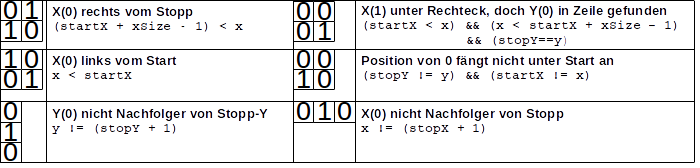
\includegraphics[scale=0.8]{mismatches.png}

Werden diese Muster nicht erkannt, aber schwarze Pixel erkannt, dann existiert ein Rechteck (\texttt{FoundOne}). Andernfalls werden nicht zuzuordnende schwarze Pixel (\texttt{Mismatch}) oder gar keine schwarzen Pixel (\texttt{Nothing}) im Bild gefunden.

Nachdem jeder Prozess sein Teilbild bearbeitet hat muss ein ausgezeichneter Hauptprozess (\texttt{Master}) alle Ergebnisse zusammenfassen, dies geschieht in folgenden Schritten.

\begin{enumerate}
	\item Gibt es ein Teilbild mit schwarzen Pixeln, welche aber kein Rechteck bilden, dann kann direkt abgebrochen werden mit: \texttt{Mismatch}.
	\item Wenn alle Teilbilder \texttt{Nothing} finden, dann kann auch abgebrochen werden mit \texttt{Nothing}.
	\item Gibt es nur ein \texttt{FoundOne} und sonst \texttt{Nothing}, kann das Rechteck ausgegeben werden.
\end{enumerate}

Falls mehrere \texttt{FoundOne} vorliegen und vorher nicht abgebrochen wurde muss der \texttt{Master} überprüfen ob die gefundenen Rechtecke zusammenhängend sind, dies kann durch folgende Kriterien überprüft werden.

\begin{enumerate}
	\item Die Start- \& Stop-X Werte stimmen bei jedem Rechteck überein.
	\item Bis auf dem ersten Prozess der ein Rechteck in einer Zeile gefunden hat, müssen alle schwarze Pixel in ihrer ersten Zeile finden.
	\item Bis auf dem letzten Prozess der ein Rechteck gefunden hat, müssen alle schwarzen Pixel in ihrer letzten Zeile finden.
\end{enumerate}

Nach dieser letzten Überprüfung kann der Master-Prozess das Ergebnis ermitteln und die Start- \& Stopp-Koordinaten des gefundenen Rechtecks ausgeben. 

Durch die Betrachtung der Umsetztung stellt man fest, dass für den Algorithmus ein Best-Case darin besteht sofort ein \texttt{Mismatch} zu finden, da direkt abgebrochen werden kann. Der Average-Case stellt ein Digitalbild ohne schwarze Pixel dar, da nach überprüfen aller Pixel abgebrochen werden kann, aber keine weiteren Überprufungen stattfinden. Der Worst-Case besteht darin mehrere Rechtecke zu finden, da alle Rechtecke zusammenhängend sein müssen. Für die Untersuchungen zur Laufzeit werden, stets diese drei Fälle berücksichtigt.


\subsection{Verwendung}
\subsubsection{Ausführung}
Der Quellcode kann mit Hilfe des folgenden Aufrufs auf dem PC oder dem Cluster kompiliert werden:

\begin{itemize}
	\item \texttt{cmake CMakeLists.txt -DCMAKE\_BUILD\_TYPE=RELEASE \&\& make}
\end{itemize}

Mif folgenden Befehl wird das Programm auf 4 Prozessoren ausgeführt:

\begin{itemize}
	\item \texttt{mpirun -npernode 4 rectanglePatternDetection} \textbf{FILE}
\end{itemize}

Für das Programm können Kommandozeilenargumente zur Angabe des Konfigurationsfiles zur Erstellung des zu untersuchenden Digitalbildes angegeben werden.

\subsubsection{Konfigurationsfile}
Die Anwendung unterstützt drei Modi zur Erzeugung des Digitalbildes, welcher dieser Modi verwendet wird, steht immer in der ersten Zeile des Files.

\paragraph{Modi 2 - Custom Mode}Der \texttt{Custom Mode} ermöglicht die direkte angabe einer n*n Matrix aus Nullen und Einzen.

TODO: Beschreibe dass Modi 0 und 1 die Eingabe mit der Angabe von n und der Hintergrundfarbe gemeinsam verwenden 

TODO: beschreibe die Erzeugung von Rechtecken mittels Mode 0 und die Erzeugung von einzelnen Punkten durch Mode 1

%Speed-Up , Effizienz
%Wo liegt das Maximum für das zu untersuchende quadratische Raster?
%Kommunikationsoverhead
\subsection{Laufzeitverhalten}
% Auswertungsoverhead durch Master (Auswertung von Gather - parallel)

\subsubsection{Festes n}
\begin{tikzpicture}
\begin{axis}
[            axis x line=middle,
            axis y line=middle,
            enlarge y limits=true,
            width=15cm, height=8cm,     % size of the image
            grid = major,
            grid style={dashed, gray!30},
            ylabel=Time in s,
            xlabel=n,
            legend style={at={(0.1,-0.1)}, anchor=north}
]
\addplot[black, mark=x] table [x=n, y=T2 , col sep=space] {../rectangle/measures/nScaling/88/measure0.csv};
\addplot[blue, mark=*] table [x=n, y=T2 , col sep=space] {../rectangle/measures/nScaling/88/measure1.csv};
\addplot[red, mark=+] table [x=n, y=T2 , col sep=space] {../rectangle/measures/nScaling/88/measure2.csv};
\legend{0,1,2}
\end{axis}
\end{tikzpicture}

\begin{tikzpicture}
\begin{axis}
[            axis x line=middle,
            axis y line=middle,
            enlarge y limits=true,
            width=15cm, height=8cm,     % size of the image
            grid = major,
            grid style={dashed, gray!30},
            ylabel=Time in s,
            xlabel=n,
            legend style={at={(0.1,-0.1)}, anchor=north}
]
\addplot[black, mark=x] table [x=n, y=T2 , col sep=space] {../rectangle/measures/nScaling/44/measure0.csv};
\addplot[blue, mark=*] table [x=n, y=T2 , col sep=space] {../rectangle/measures/nScaling/44/measure1.csv};
\addplot[red, mark=+] table [x=n, y=T2 , col sep=space] {../rectangle/measures/nScaling/44/measure2.csv};
\legend{0,1,2}
\end{axis}
\end{tikzpicture}
\subsubsection{Festes p}
\begin{tikzpicture}
\begin{axis}
[            axis x line=middle,
            axis y line=middle,
            enlarge y limits=true,
            width=15cm, height=8cm,     % size of the image
            grid = major,
            grid style={dashed, gray!30},
            ylabel=Time in s,
            xlabel=hosts,
            legend style={at={(0.1,-0.1)}, anchor=north}
]
\addplot[black, mark=x] table [x=hosts, y=T1 , col sep=space] {../rectangle/measures/processorScaling/44/40000/measure0.csv};
\addplot[blue, mark=*] table [x=hosts, y=T1 , col sep=space] {../rectangle/measures/processorScaling/44/40000/measure1.csv};
\addplot[red, mark=+] table [x=hosts, y=T1 , col sep=space] {../rectangle/measures/processorScaling/44/40000/measure2.csv};
\legend{0,1,2}
\end{axis}
\end{tikzpicture}

\begin{tikzpicture}
\begin{axis}
[            axis x line=middle,
            axis y line=middle,
            enlarge y limits=true,
            width=15cm, height=8cm,     % size of the image
            grid = major,
            grid style={dashed, gray!30},
            ylabel=Time in s,
            xlabel=hosts,
            legend style={at={(0.1,-0.1)}, anchor=north}
]
\addplot[black, mark=x] table [x=hosts, y=T2 , col sep=space] {../rectangle/measures/processorScaling/88/40000/measure0.csv};
\addplot[blue, mark=*] table [x=hosts, y=T2 , col sep=space] {../rectangle/measures/processorScaling/88/40000/measure1.csv};
\addplot[red, mark=+] table [x=hosts, y=T2 , col sep=space] {../rectangle/measures/processorScaling/88/40000/measure2.csv};
\legend{0,1,2}
\end{axis}
\end{tikzpicture}
\subsection{Fazit}

\pagebreak

\section{Projektaufgabe 2: Numerische Integration mittels Parabelformel}
\lstset{language=Fortran,frame=none, keepspaces=false, basicstyle=\footnotesize,showstringspaces=false}  
In diesem Abschnitt wird auf die Projektaufgabe 2 eingegangen.
Zunächst wird im \autoref{ref:verwendung} kurz erklärt wie das Programm kompiliert und gestartet wird sowie auf die Kommandozeilenargumente eingegangen.
Im Anschluss wird die Realisierung und damit die Lösung des Problems im \autoref{ref:realisierung} betrachtet.
Anschließend erfolgt im \autoref{ref:ergebnisse} die Auswertung der Realisierung.
Im letzten \autoref{ref:fazit} wird ein Fazit zu der Aufgabe gezogen.

\subsection{Verwendung}
\label{ref:verwendung}
Der Quellcode kann mit Hilfe folgendes Aufrufes auf dem MC-3-System kompiliert werden:
\begin{itemize}
	\item f77.px -o A2star.px A2star.f
\end{itemize}
Mit folgendem Befehl wird das Programm ausgeführt:
\begin{itemize}
	\item run -f0 4 2 A2star.px \textbf{funktion} \textbf{n}
\end{itemize}

Für das Programm können Kommandozeilenargumente zur Auswahl der Testfunktion und die Größe der zu berechnenden Teilstücke des Integrals angegeben werden.
\paragraph{funktion:}
Das Programmargument \textbf{funktion} entscheidet darüber, welche der beiden gegebenen Testfunktionen verwendet wird.
Als gültige Eingabe wird 1 für Funktion 1 und 2 für Funktion 2 erwartet.
\paragraph{n:}
Das zweite Programmargument \textbf{n} gibt die 2er Potenz der zu berechnenden Teilstücke des Integrals an.
Je größer das \textbf{n}, umso genauer wird das berechnete PI.
De höchstmöglichste zulässige Eingabe ist 20, das sind 1048576 zu berechnende Teilstücke.
Diese Vorgehensweise soll zum Einen sicher stellen, dass \textbf{n} stets durch 2 Teilbar ist und zum Anderen das Laufzeitmessen vereinfachen, da ein exponentielles Wachstum vorliegt.
Sollte kein Programmargument angeben werden, so wird intern die Funktion 1 mit $n = 2^{15} = 32768$ verwendet.

Weiterhin wird eine ungerade Prozessorzahl ausgeschlossen, damit stets gewährleistet ist, dass die zu berechnende Anzahl an Teilstücke pro Prozessor eine ganzzahlige Zahl ist.

\subsection{Realisierung}
\label{ref:realisierung}
Grundlegend wurde sich bei der Realisierung für eine Stern-Topologie entschieden.
Gewählt wurde diese Topologie, da bei der Parallelisierung dieser Aufgabe ein Master existert, welche alle Teilergebnisse empfängt und summiert.
Weiterhin wurde diese Topologie bereits in einem Seminar implementiert.
Wie die Topologie erstellt wird zeigt \autoref{ref:top}.

\begin{lstlisting}[caption=Erzeugen der Stern-Topologie\label{ref:top}]
	if(id.eq.0) then
		do i=1,(np-1)
			links(i)=addnewlink(topid,i,1)
		enddo
	else
		link=addnewlink(topid,0,1)
	endif
\end{lstlisting}

Bedingt durch die Realisierung als Kommandozeilenparameter, entfällt der Kommunikationsoverhead für das Verteilen von \textbf{n} und \textbf{funktion}.
Daher kennen alle Prozessoren \textbf{n} sowie die Testfunktion beim Programmstart.

Die Prozessoren können explizit ihre eigenen Bereich für die Teilstücke bestimmen und somit die numerische Berechnung durchführen.
Nach Abschluss der Berechnungen, werden diese an den Master-Prozessor gesendet.
Der Master-Prozessor summiert die Ergebnisse der anderen Prozessoren zu seinem eigenem Ergebnis auf und wendet die Multiplikation h/3 auf das Gesamtergebnis an.
Im Anschluss werden die Ergebnisse wie Referenzwert-PI, Berechnetes-PI, Abweichung und Laufzeit (nicht im Listng dargestellt) ausgegeben. 
Das folgende \autoref{ref:main} zeigt dies.

\begin{lstlisting}[caption=Empfangen und Auswerten\label{ref:main}]
c	starte die Integration
	call startIntegration(f,n,integral,h)
	if(id.eq.0) then
		print*,"use f:",f," with n:",n
c  	Integralteilstück vom Master
		summe = integral
		do i=1,(np-1)
c 	Empfange alle Teilstücke und addiere Sie
			call recv(topid,links(i),integral,8)
			summe = summe + integral
		enddo
		summe = h/3 *summe
		derivation =  PI() - summe
		print*,"--------------------------"
		print*,"PI Referece:",PI()                   
		print*,"PI Integral:",summe
		print*,"PI Derivat.:",derivation
	else
c	Sende Integralteilstücke zum Master
		call send(topid, link,integral,8)
	endif
\end{lstlisting}

Die numerische Berechnung des Integrals wird durch jeden Prozessor ausgeführt, aber jeder Prozessor führt nur einen Teil der kompletten Berechnung aus.
Die eigentliche Berechnung ist in dem \autoref{ref:intervall} zu sehen.
Zunächst berechnet jeder Prozessor die Anzahl der durchzuführenden Berechnungen, als lokales \textbf{n} (\textbf{nL}).
Im Anschluss werden Startpunkt (\textbf{aL}) und Endpunkt (\textbf{bL}) ermittelt.
Die Funktionswerte von \textbf{aL} und \textbf{bL} der Testfunktion werden addiert und in einer Summe gespeichert.
Im Anschluss werden die Zwischenstücke mit entsprechendem Faktor berechnet und ebenfalls summiert.
Die Variable \textbf{h} gibt dabei die allgemeine Schrittweite an und \textbf{step} die derzeitigen Schrittwert.

Nach erfolgter Berechnung sendet jeder Prozessor sein Ergebnis an den Master (falls der Prozessor nicht selbst der Master ist)

\begin{lstlisting}[caption=Berechnen der relevanten Bereiche für jeden Prozessor\label{ref:intervall}]
	id = myprocid() 
	nL = n / nprocs()
	aL = a + id * nL * h
	bL = aL + nL * h
c	Randwerte, getVal liefert Funktionswert der Testfunktion
	summe = getVal(f,aL) + getVal(f,bL)   
	step = aL + h
c 	Berechnung zwischenstücke, factor alterniert mit 2 und 4
	do i=1,nL-1
		exponent = mod(i,2) + 1
		factor=2**exponent
		summe = summe + dble(getVal(f,step) * factor)
		step = step + h    
	enddo
\end{lstlisting}

\subsection{Ergebnisse}
\label{ref:ergebnisse}
%TODO Tabellen

\subsubsection{Testfunktionen}

Für die Testfunktionen wird folgender Referenzwert verwendet: 3.141592653589793.
Die \autoref{ref:piP} zeigt die Abweichung zum Referenzwert von Pi bei einer konstanten Prozessoranzahl von 8 und einem sich verändernden \textbf{n}.
Die \autoref{ref:piN} zeigt ebenfalls die Abweichung, aber hier wird ein konstantes \textbf{n} von 32768 verwendet und die Prozessoranzahl variiert.

Wie in den Tabellen zu sehen ist liefert die Testfunktion 2 schneller bessere Pi-Näherungswerte als Funktion 1.
Ein Grund dafür das Funktion 1 schlechte Näherungswerte liefert liegt unter anderem an der Oberegrenze.
Diese Obergrenze ist Pi selbst.
Zusätzlich sind in der Funktion 1 die Schrittweiten bedeutend größer, als bei der Funktion 2, daher benötigt die Funktion ein größeres \textbf{n} um mehr Teilstücke berechnen zu können und somit ein genaueres Ergebnis zu liefern.

%TODO hat das was mit Arctan zu tun???
%TODO Unterschiede Genauigkeit der Funktionen mit Begründung

\begin{figure}[h]
\begin{minipage}{0.45\textwidth}
	\pgfplotstabletypeset[col sep=space
	,every head row/.style={before row={\hline},after row=\hline}
	,every last row/.style={after row=\hline}
	,every even column/.style={column type/.add={|}{|}}
	,columns={n,Abweichung-F1,Abweichung-F2}
	]{../integration/functionDiffp8.csv} 
	\caption{Mit 8 Prozessoren}
	\label{ref:piP}
\end{minipage}
\hfill
\begin{minipage}{0.45\textwidth}
	\pgfplotstabletypeset[col sep=space
	,every head row/.style={before row={\hline},after row=\hline}
	,every last row/.style={after row=\hline}
	,every even column/.style={column type/.add={|}{|}}
	,columns={p,Abweichung-F1,Abweichung-F2}
	]{../integration/functionDiffn.csv}
	\caption{Mit n = 32768}
	\label{ref:piN}
\end{minipage}
\end{figure}



%Speed-Up , Effizienz
\subsubsection{Laufzeitverhalten}
\paragraph{Festes n}
\paragraph{Festes p}

\subsection{Fazit}
\label{ref:fazit}
Kommunikationsoverhead spielt hier eine untergeordnete Rolle, da Minimum an Kommunikation zur Berechnung notwendig ist.
%TODO
Weiterhin lohnt sich die Parallelisierung,..


%\appendix
%\section{Quellcode Aufgabe 1}
%
%\section{Quellcode Aufgabe 2}
%\lstset{language=Fortran,numbers=left, keepspaces=false, basicstyle=\footnotesize,showstringspaces=false} 
%\lstinputlisting[]{../integration/A2star.f}

\end{document}
